\section{Logs}\label{sec:logs-storing}

El següent conjunt de paràmetres és el que permet agrupar tota la informació present als logs.
L’evolució durant els anys no ha afectat gaire respecte als paràmetres existents sinó al contingut d’aquests. \\

\noindent
Aquí un exemple d’un \textit{log}:

\begin{itemize}
    \item \texttt{ip\_address:  39.92.248.6}
    \item \texttt{date: 20/Apr/2011}
    \item \texttt{time: 23:59:59 +0200}
    \item \texttt{request}:
    \begin{itemize}
        \item \texttt{method: GET}
        \item \texttt{resource: /e-prints/bitstream/2117/8469/1/sdarticle.pdf}
        \item \texttt{version: HTTP/1.0}
        \item \texttt{status\_code: 304}
        \item \texttt{response\_size: -}
    \end{itemize}
    \item \texttt{referer: null}
    \item \texttt{user\_agent:  gsa-crawler (Enterprise; T2-QGG2U8NZXNSAA upcnet\\.backoffice.aps@upcnet.es)}
\end{itemize}


\noindent \\
Aquesta estructura de dades representa la informació que podem extreure directament dels \textit{logs} provenents d'\gls{UPCommons}.
El resultat del nostre processament d'aquests, altera aquest format per afegir més informació, com veurem més endavant.

\clearpage

\subsection{Bases de dades candidates}\label{subsec:log-db-options}

\noindent \\
A continuació llistarem una sèrie d’opcions candidates a ser el sistema gestor de bases de dades on emmagatzemarem tots els logs.

\noindent \\
La majoria són sistemes d’agregació de logs, que incorporen eines de monitoratge, sistemes d’alertes, visualització, etc.
És criteri nostre fer-ne ús d’aquests serveis o només continuar amb la base de dades.

\noindent \\
Com a primeres opcions considerem aquelles que siguin de programari lliure i en les quals puguem instal·lar la base de dades de forma local.

\noindent \\
\textbf{Grafana Loki~\cite{loki:main}}\label{subsubsec:log-db-option-loki}

\noindent \\
\textit{Grafana Labs} proporciona \textit{Loki}, un sistema d’agregació codi obert de logs basat en Prometheus.
És un sistema distribuït i dissenyat per ser escalable.
Les seves característiques principals:

\begin{itemize}
    \item \textbf{Escalabilitat}: disposa de diferents modes de desplegament on pots escollir el que més s’adapti pels teus requisits.
    \item \textbf{Integració}: suporta diverses implementacions/llibreries de tercers per fer-ne servir, i diversos modes de desplegament en local.
    \item \textbf{Grafana}: integració per defecte amb \textit{Grafana} com a eina principal d’observabilitat.
    \item \textbf{Emmagatzemament}: Loki només indexa les metadades dels logs~\cite{loki:indexing}, és a dir, només el \textit{timestamp} i els \textit{labels} definits.
    El contingut del log no s’indexa.
    Utilitzant aquest plantejament, s’aconsegueix reduir la quantitat total de disc necessari.
    \begin{itemize}
        \item Aquesta característica és bastant interessent si utilitzem aquests labels per afegir informació relacionada amb el recurs accedit per després com a millorar el procés de cerca.
    \end{itemize}
\end{itemize}

\clearpage

\noindent
\textbf{Elastic~\cite{elastic}}

\noindent \\
Elastic, conegut pel seu motor de cerca Elasticsearch, disposa d’una solució de monitoratge de logs.
Les seves característiques principals:

\begin{itemize}
    \item \textbf{Escalabilitat}: dissenyat per monitorar logs fins a una escala de petabytes
    \item \textbf{Integració}: suporta diverses implementacions/llibreries de tercers per fer-ne servir, i modes de desplegament en local.
    \item \textbf{\textit{Logstash}}: mecanisme per centralitzar i transformar les dades per després emmagatzemar-les a qualsevol lloc.
    \item \textbf{\textit{Kibana}}: integració per defecte amb \textit{Elastic Kibana} com a eina principal d’observabilitat.
    \item \textbf{Categorització}: incorpora una eina per identificar patrons, tendències i anomalies als logs.
\end{itemize}


\noindent \\
\textbf{Apache SOLR~\cite{SOLR}}

\noindent \\
Apache SOLR és una plataforma de cerca que es pot utilitzar com a mecanisme d’emmagatzemament de documents. 
Les seves característiques principals:

\begin{itemize}
    \item \textbf{Escalabilitat}: basat en un sistema distribuït i basat en rèpliques, és optimitzat per grans volums de dades.
    \item \textbf{Integració}: la comunicació amb el servei es realitza mitjançant l’\gls{API} de SOLR sobre \gls{HTTP} .
    També suporta diferents modes de desplegament en local.
    \item \textbf{Lucene}: fa servir \textit{Apache Lucene} com a motor de cerca principal.
\end{itemize}

\noindent
Com a contrapartida:

\begin{itemize}
    \item \textbf{Visualització}: no disposa d’un sistema de visualització de dades per defecte, així doncs caldria emprar-ne un de tercers.
\end{itemize}


\clearpage

\noindent
Altres opcions que no són de codi obert són les següents,  la versió gratuïta que proporcionen és bastant limitada, no hi ha prou documentació a la xarxa són les següents:

\begin{itemize}
    \item \textbf{Graylog}~\cite{graylog}
    \item \textbf{Papertrail}~\cite{papertrail}
    \item \textbf{Loggly}~\cite{loggly}
    \item \textbf{Splunk}~\cite{splunk}
\end{itemize}

\clearpage

\subsection{Decisió}\label{subsec:log-db-decision}

\noindent
La primera decisió presa fou donar suport a \textit{Grafana Loki}, amb els motius que llistarem a continuació:

\begin{itemize}
    \item Base de dades de codi obert compatible per diferents plataformes.
    \item És una eina ben documentada~\cite{loki:documentation}.
    \item Té una gran quantitat d’usuaris actius.
    El repositori de codi~\cite{loki:code} és mantingut activament i de forma actual.
    \item Integració per defecte amb \textit{Grafana} per poder visualitzar els \textit{logs}.
    \item Diverses llibreries~\cite{loki:libraries} ja implementades per enviar \textit{logs} a la base de dades.
    \item Com prèviament s’ha mencionat, la indexació és a partir del \textit{\gls{timestamp}} més les metadades.
    Aquestes darreres, poden ser utilitzades per afegir valors que després agilitzaran el processament. \\ \\
    Com podem veure a la imatge~\ref{fig:loki-indexing}, converteixen un log semblant als nostres en un altre adaptat al format de loki, on utilitzen com etiqueta el tipus petició (\textit{action}) o el codi d’estat (\textit{status\_code}) \\ \\
    El nostre cas, en podem afegir uns que indiquin el tipus de \textit{log} (cerca, accés a recurs) o marcar-ne alguns que tinguin algun contingut inexacte.
\end{itemize}

\clearpage

\begin{figure}[htbp]
    \centerline{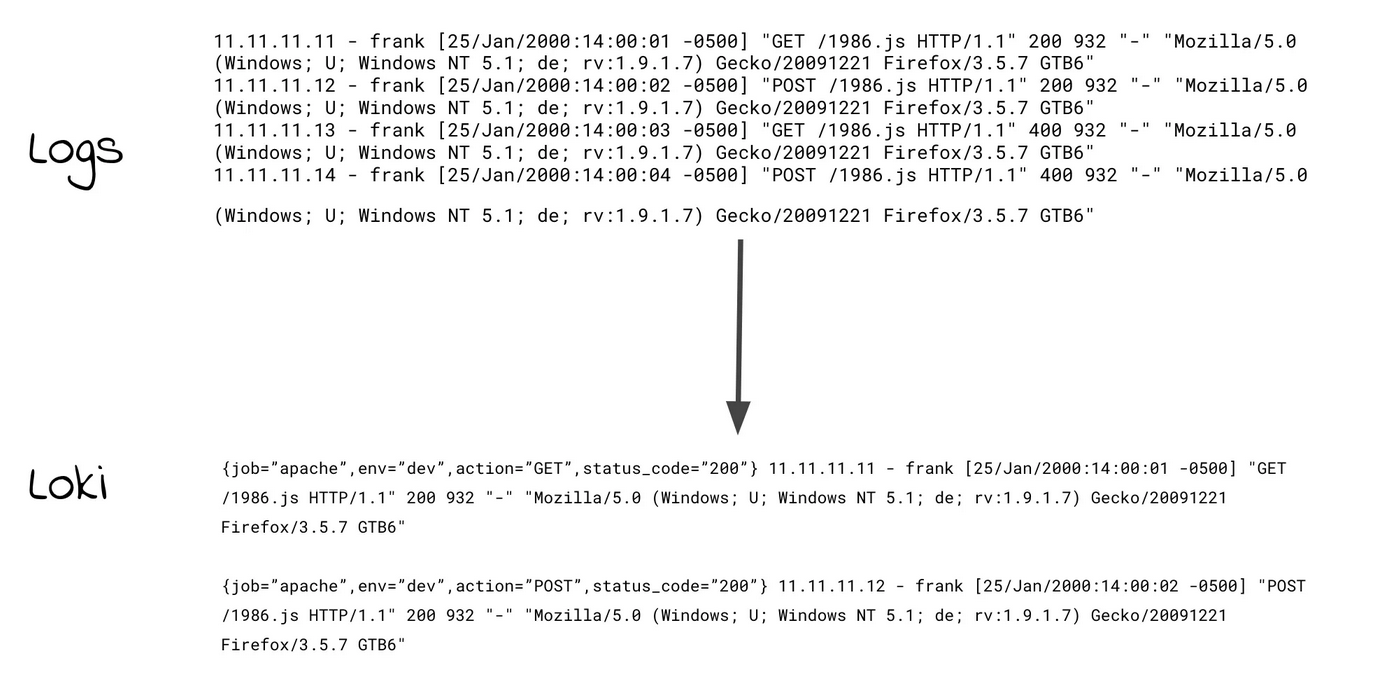
\includegraphics[width=1\textwidth]{figures/loki-indexing}}
    \captionsetup{justification=centering}
    \caption{Exemple del funcionament de la indexació dels paràmetres a \textit{Grafana Loki}.}\label{fig:loki-indexing}
    \source{\url{https://medium.com/geekculture/pushing-logs-to-loki-without-using-promtail-fc31dfdde3c6}}
\end{figure}

\noindent \\
Malauradament, errors durant l’etapa de configuració, concretament XXXXXXXXXX, ens van fer recular i considerar altres opcions.

\clearpage

\noindent
La següent opció és \textit{InfluxDb}.
Aquesta base de dades, també basada en series temporals, té característiques similars a l’anterior:

\begin{itemize}
    \item Base de dades de codi obert compatible per diferents plataformes.
    \item És una eina ben documentada~\cite{influxdb:documentation}.
    \item Té una gran quantitat d’usuaris actius.
    El repositori de codi~\cite{influxdb:code} és mantingut activament i de forma actual.
    \item Integració per defecte amb Grafana per poder visualitzar els \textit{logs}.
    \begin{itemize}
        \item Aquest és un dels punts que ens van fer considerar aquesta opció, ja que va ser recomanada pel mateix aplicatiu de Grafana.
    \end{itemize}
    \item Diverses llibreries~\cite{influxdb:libraries} ja implementades per enviar logs a la base de dades.
    \begin{itemize}
        \item En el nostre cas emprar \textit{influxdb-client}~\cite{influxdb:python} pel llenguatge \textit{Python}.
    \end{itemize}
    \item En aquest cas, però, la indexació és a partir dels tags.
    Utilitzarem aquest camp per afegir valors freqüents, que poden ser agrupats i fàcilment indexats.
\end{itemize}

\begin{figure}[htbp]
    \centerline{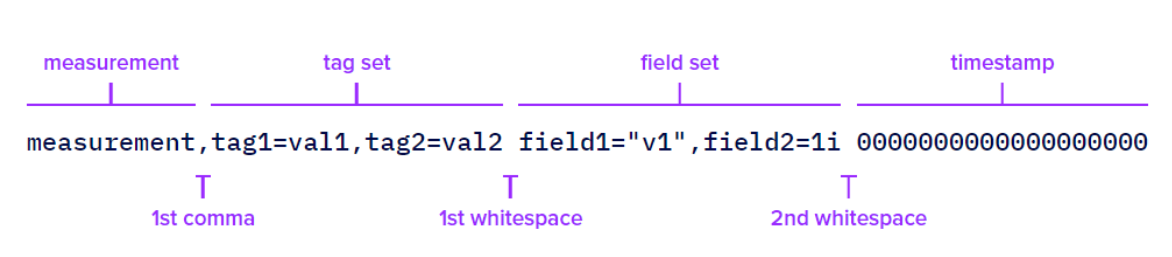
\includegraphics[width=1\textwidth]{figures/influxdb-indexing}}
    \captionsetup{justification=centering}
    \caption{Exemple del funcionament de la indexació dels paràmetres a \textit{InfluxDb}.}\label{fig:influxdb-indexing}
    \source{\url{https://docs.influxdata.com/influxdb/v2/get-started/write/#line-protocol-element-parsing}}
\end{figure}